\subsection{Creación del lienzo}\label{sec:lienzo} 
Cuando introdujimos el método de rasterización dijimos que este suele ser usado con mallas de polígonos, que a su vez estaban compuestas por puntos en un espacio afín que se unen formando caras. Lo cierto es que en IG se hace uso de múltiples espacios de coordenadas, los cuales es imprescindible conocer para entender el proceso de definición de geometría y pasamos a enumerar.
% Si bien se puede hacer \textit{raymarching} directamente sobre una escena 3D, nuestra escena constará únicamente de un plano formado por cuatro vértices y dos triángulos, que usaremos como lienzo  (o \textit{canvas}) para dibujar sobre él. Para ello, necesitaremos trabajar sobre diferentes espacios de coordenadas que pasamos a enumerar.
\begin{itemize}
    \item \textbf{Coordenadas locales o de objeto:} distancias relativas al origen del objeto.
    \item \textbf{Coordenadas globales o de mundo:} distancias relativas a un origen común para todos los objetos.
    \item \textbf{Coordenadas de cámara:} distancias relativas a un sistema de referencia posicionado y alineado con la cámara.
    \item \textbf{Coordenadas de recortado:} distancias normalizadas en el rango $[-1,1]^2$ relativas a un sistema asociado al rectángulo que forma la imagen en pantalla.
    \item \textbf{Coordenadas de dispositivo:} están centradas en la esquina inferior izquierda de la pantalla y toman valor en el rango $[0,r_x]\times [0,r_y]$, donde $r=(r_x,r_y)$ es la resolución de la pantalla.
\end{itemize}

% Si hacemos uso de \texttt{GL\_TRIANGLES} bastará con definir los vértices en sentido antihorario, pero hay que tener en cuenta que tendremos que repetir dos vértices, ya que se irán formando los triángulos en grupos de tres vértices. Una alternativa para no repetir vértices sería utilizar tablas de vértices e índices, pero en nuestro caso no merece la pena al tener únicamente seis vértices. Un ejemplo de definición de vértices formando un lienzo rectangular podría ser el que se muestra en la \autoref{fig:canvas}.\newline

% \begin{figure}[ht]
%     \centering
%     \begin{minipage}{0.50\textwidth}
%         \begin{lstlisting}
% glBegin(GL_TRIANGLES);
%     glColor3f(1.0f, 1.0f, 1.0f); 
    
%     // Triangulo inferior
%     glVertex3f(-2.0f, -1.0f, 0.0f);
%     glVertex3f(-2.0f, 1.0f, 0.0f);
%     glVertex3f(2.0f, 1.0f, 0.0f);
    
%     // Triangulo superior
%     glVertex3f(-2.0f, -1.0f, 0.0f);
%     glVertex3f(2.0f, 1.0f, 0.0f);
%     glVertex3f(2.0f, -1.0f, 0.0f);
% glEnd();
% \end{lstlisting}
%     \end{minipage}%
%     \hfill
%     \begin{minipage}{0.40\textwidth}
%         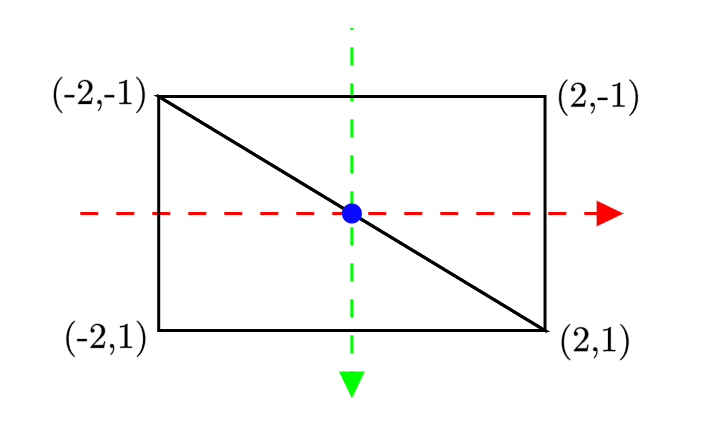
\includegraphics[width=\textwidth]{canvas.png}
%     \end{minipage}
    
    
%     \caption{Construcción del lienzo}
%     \label{fig:canvas}
% \end{figure}
Dado que para usar rasterización el lienzo deberá estar definido como una malla de polígonos, deberemos declarar los vértices que la conforman y cómo estos se unen formando primitivas, en este caso triángulos. Este lienzo, como toda geometría, tendrá asignado dos \textit{shaders} o procesadores, que son programas que se ejecutan en la GPU. Estos programas pueden recibir parámetros, pero son independientes entre sí, siendo la única forma en la que pueden comunicarse entre ellos mediante el paso de atributos de entrada y salida. Hay dos tipos de \textit{shaders}: de vértices (\textit{vertex shader}) y de fragmentos o pixels (\textit{fragment shader}), cada uno con atributos específicos de entrada y salida.\newline

En el \textit{vertex shader} utilizaremos los siguientes atributos.
\begin{itemize}
    \item $v_{loc}$: vector de cuatro flotantes que contiene las coordenadas
    homogéneas locales del vértice a procesar. La cuarta componente es la componente homogénea, que es necesaria para realizar el cambio a coordenadas recortadas. Se trata de un parámetro de entrada enviado por la aplicación al visualizar una secuencia de vértices.
    \item $v_{wc}$: vector de cuatro flotantes con la posición transformada del vértice actual. El objetivo del \textit{vertex shader} es el de calcular su valor, luego es un parámetro de salida. 
    % \item \textbf{\texttt{in vec4 gl\_Vertex}}: contiene las coordenadas locales del vértice actual y es pasado autómaticamente por la aplicación. 
    % \item \textbf{\texttt{out vec4 gl\_Position}}: posición transformada del vértice actual que deberemos calcular. La cuarta componente es la componente homogénea, que es necesaria para realizar el cambio a coordenadas recortadas.
\end{itemize}
Por otro lado, en el \textit{fragment shader} usaremos los que siguen.
\begin{itemize}
    \item $v_{frag}$: vector de cuatro flotantes con las coordenadas de dispositivo para el centro del píxel actual. Es un atributo de entrada, los cuales interpolan su valor automáticamente en cada vértice en los \textit{fragment shaders}. La cuarta componente es la inversa de la componente homogénea de $v_{rec}$, y se utiliza en el cálculo de la profundidad de los pixels y en las operaciones de corrección de perspectiva.
    \item $v_{col}$: terna RGBA de flotantes que contendrá el color del píxel actual. Es un parámetro de salida, y la función del \textit{fragment shader} es otorgarle un valor.
    % \item \textbf{\texttt{in vec4 gl\_FragCoord}}: coordenadas de dispositivo para el centro del píxel actual en el \textit{fragment shader}. Al ser un atributo de entrada del \textit{fragment shader}, está interpolada en cada vértice. La cuarta componente es la inversa de la componente homogénea de \texttt{gl\_Position}, y se utiliza en el cálculo de la profundidad de los pixels y en las operaciones de corrección de perspectiva.
    % \item \textbf{\texttt{out vec4 gl\_FragColor}}: terna RGBA que asignaremos como color del píxel actual en el \textit{fragment shader}.
\end{itemize}
% Adicionalmente, podremos pasar nuestros propios atributos desde otro programa si estos son de cierto tipo
% Por último, en caso de que queramos pasar nuestros propios atributos desde otro programa, deberemos hacerlo a través de un \texttt{uniform}.\newline

En primer lugar se ejecuta una instancia del \textbf{procesador de vértices o \textit{vertex shader}} para cada vértice de la geometría. Su finalidad es realizar transformaciones de coordenadas, y adicionalmente pasar atributos al \textit{fragment shader}. Dada la posición del vértice actual, que se nos proporciona a través del atributo $v_{loc}$, para cambiar de un sistema de coordenadas a otro se utilizan matrices de transformación \cite{article:matrices} \cite{article:matrices2}. Todas ellas son de flotantes con dimensión $4\times 4$, y haremos uso de las siguientes.
\begin{figure}[h]
    \centering
    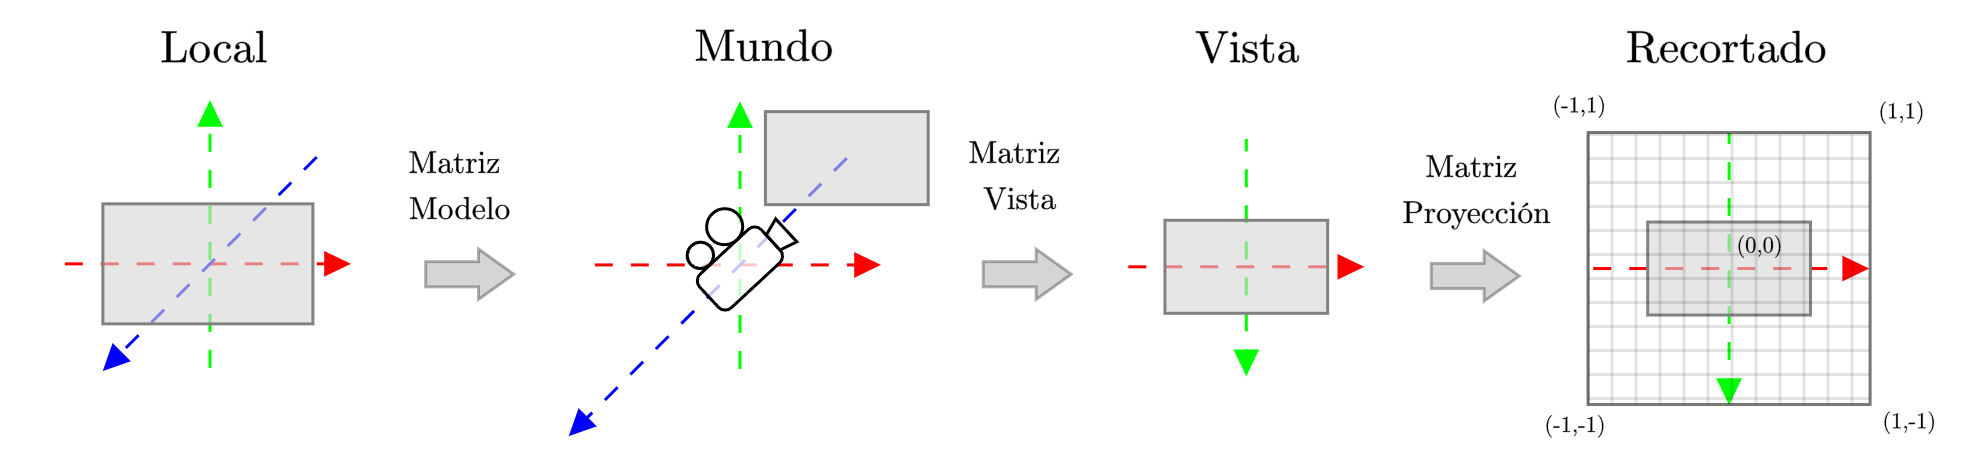
\includegraphics[width=\textwidth]{Plantilla-TFG-master/img/matrices2.png}
    \caption{Coordenadas locales a recortadas}
    \label{fig:matrices}
\end{figure}
\begin{itemize}
    \item \textbf{Matriz de modelo $\boldsymbol{M}$:} define la posición, orientación y escala del objeto en la escena. Se utiliza para pasar del coordenadas locales a coordenadas de mundo. En nuestro caso, si creamos el plano centrado en el origen, podemos simplemente tomar la matriz identidad de dimensión cuatro
    \begin{equation*}
        M = Id_{4\times 4}.
    \end{equation*}
    \item \textbf{Matriz de vista  $\boldsymbol{V}$:} define la posición y orientación de cada punto respecto a la cámara de la escena. Se utiliza para pasar de coordenadas de mundo a coordenadas de vista. Lo que ocurre en realidad es que la cámara está fija en el origen, y es el resto de la escena es la que se mueve respecto a ella. Por tanto, esta matriz contiene la posición y orientación inversa de la cámara. En nuestro caso, si queremos desplazar la cámara una unidad en el eje Z, la matriz de vista tendrá la forma
    \begin{equation*}
        V = \begin{pmatrix}
        1 & 0 & 0 & 0\\
        0 & 1 & 0 & 0\\
        0 & 0 & 1 & -1\\
        0 & 0 & 0 & 1
        \end{pmatrix}.
    \end{equation*}
    
    \item \textbf{Matriz de proyección:} define cómo la escena se proyecta en la pantalla, incluyendo el campo de visión, aspecto y planos cercano y lejano. Se utiliza para pasar de coordenadas de vista a coordenadas recortadas en función de las siguientes características del \textit{view-frustum}, la región del espacio de la escena que es visible por pantalla.
    \begin{itemize}
        \item Apertura vertical del campo de visión $\beta$ indicada como un ángulo entre $0$ y $180$ grados.
        \item Relación de aspecto $a$ entre el ancho $w$ y el alto $h$ del \textit{view-frustrum}.
        \item Límites cercano y lejano en el eje $Z$ cambiados de signo $n$ y $f$ del \textit{view-frustrum}.
    \end{itemize}
    La matriz se construye como
    \begin{equation*}
        M_P = \begin{pmatrix}
        \frac{c}{a} & 0 & 0 & 0\\
        0 & c & 0 & 0\\
        0 & 0 & \frac{n+f}{n-f} & \frac{2nf}{n-f}\\
        0 & 0 & -1 & 0
        \end{pmatrix}, \text{ donde } c = \coth\left({\frac{\beta}{2}}\right).
    \end{equation*}

    % \item \textbf{Matriz de ventana o \textit{viewport}:} se transforman las coordenadas de recortado a las coordenadas de dispositivo. Estas coordenadas están centradas en la esquina inferior izquierda de la pantalla y están en el rango $[0,r_x]\times [0,r_y]$, donde $r=(r_x,r_y)$ es la resolución de la pantalla.
\end{itemize}

\begin{figure}[ht!]
    \centering
    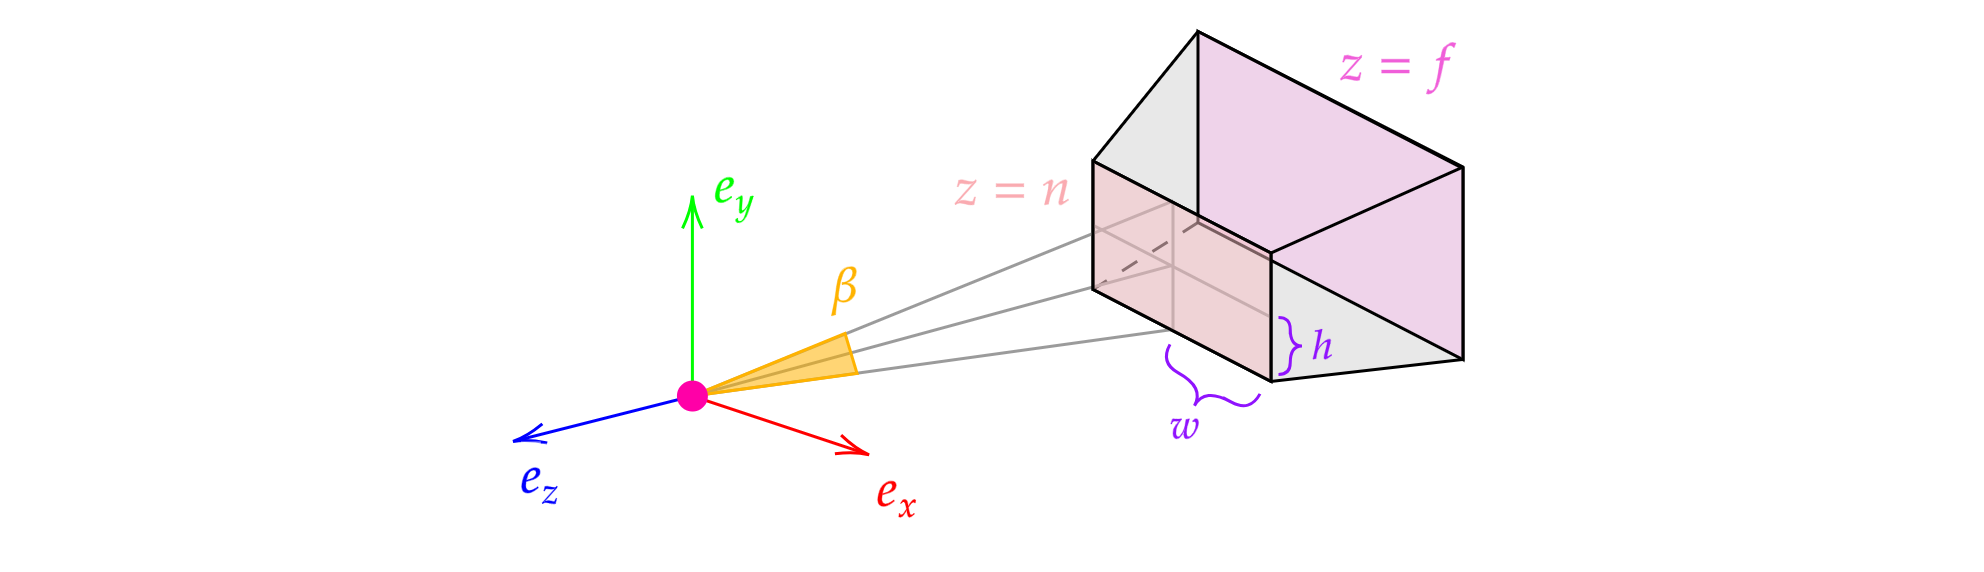
\includegraphics[width=\textwidth]{Plantilla-TFG-master/img/frustrum.png}
    \caption{Parámetros del \textit{view frustrum}}
\end{figure}

Con esta información ya podemos escribir nuestro \textit{vertex shader}, mostrado en la \autoref{fig:mainVS}.  
\begin{figure}[ht!]
    \centering
       \begin{algorithm}[H]
            \caption{Vertex Shader}
            \KwData{matriz de proyección $M_P$, matriz de vista $M_V$, matriz de modelo $M_M$, y coordenadas locales homogéneas del vértice $v_{loc}$}
            \KwResult{posición transformada del vértice actual en coordenadas homogéneas de mundo $v_{wc}$}
                $v_{wc} \gets M_P \cdot M_V \cdot M_M \cdot v_{loc}$
        \end{algorithm}
    \caption{Cuerpo del método \texttt{main} del \textit{vertex shader}}
    \label{fig:mainVS}
\end{figure}

Tras la ejecución del \textit{vertex shader} las coordenadas de recortado se transforman a coordenadas de dispositivo, que el \textbf{procesador de fragmentos o \textit{fragment shader}} recibirá como entrada. De él se ejecutará una instancia para cada píxel de la pantalla, y su objetivo es asignar a la variable $v_{loc}$ el color que el píxel tendrá como una terna RGBA, y será aquí donde hagamos todos los cálculos necesarios pare renderizar la superficie con \textit{spheretracing}. El primer paso para esto será definir un sistema de coordenadas dentro del propio lienzo con el que sea más cómodo trabajar que con el que ya disponemos a través de $v_{frag}$.\newline

Para obtener estas coordenadas, primero desplazamos el origen que nos proporciona $v_{frag}$ al centro de la pantalla usando el número de columnas y filas de pixels en la imagen, que deberemos pasar como parámetro al \textit{shader} y llamaremos \texttt{u\_resolution}, para posteriormente normalizar respecto a alguno de los ejes. Hacemos esto porque si intentamos normalizar sobre ambos ejes obtendremos coordenadas en el rango $[-0.5,0.5]^2$, y al no ser (en general) el lienzo cuadrado, la imagen se verá estirada en la dirección del eje más largo. Nosotros normalizaremos respecto al eje vertical, ya que en nuestro caso será siempre el menor. Esto nos dará como resultado unas coordenadas con valores en $\left[ -0.5\cdot aspect, 0.5\cdot aspect \right] \times [-0.5, 0.5]$, donde $aspect$ es el ratio de aspecto del lienzo, el resultado de dividir el ancho de la imagen por el alto, ambos medidos en pixels. Finalmente, para que la coordenada Y tome siempre valores en $[-1,1]$ multiplicamos por dos. Con esto conseguimos las coordenadas del centro del pixel en coordenadas normalizadas de dispositivo, similares a las de recortado pero divididas por la componente homogénea.
\begin{equation*}
    uv = \frac{2\cdot(v_{frag} - 0.5\cdot u\_resolution)}{u\_resolution_y}.
\end{equation*}

Hemos denotado a las coordenadas obtenidas como $uv$, haciendo referencia a la similitud que tienen con el uso que se le da a las coordenadas de textura habituales, ya que las vamos a usar para pintar sobre el lienzo como si de aplicar una textura se tratase. Cuando se trabaja con \textit{fragment shaders} la forma de debugear es dando colores a los pixels. En nuestro caso, podemos ver la diferencia entre ambos sistemas de coordenadas si usamos $uv$ como los canales rojo y verde del parámetro de salida $v_{col}$, superponiendo una rejilla construida usando la función módulo para apreciar si existe deformación, tal y como se muestra en la \autoref{fig:uv}. En ella podemos observar que si normalizamos sobre el eje horizontal, los verdes y amarillos no llegan a ser del todo intensos, ya que la componente del verde (la vertical) no llega a su valor máximo. Normalizando ambos ejes obtenemos el rango de colores completo, pero existe deformación en la rejilla debido a que el lienzo no es cuadrado. Finalmente, normalizando sobre el eje vertical obtenemos también el rango completo de colores, ya que los valores del eje horizontal que se salen del rango $[-1,1]$ son visualizados como si hubieran sido acotados en dicho intervalo, pero la rejilla se dibuja correctamente. En las siguientes secciones veremos cómo usar estas coordenadas para dibujar nuestra superficie sobre el lienzo.
\newline

\begin{figure}[htbp]
    \centering
    \begin{minipage}[b]{0.45\textwidth}
        \centering
        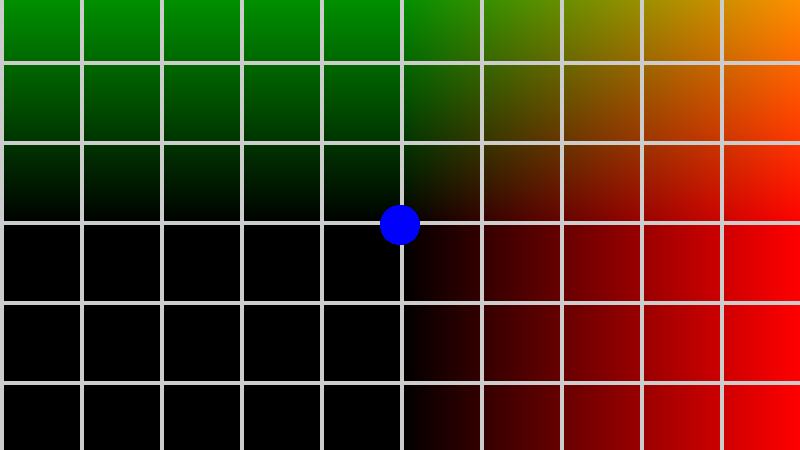
\includegraphics[width=\textwidth]{Plantilla-TFG-master/img/normX.png}
        \caption{Eje X}
    \end{minipage}
    \hfill
    \begin{minipage}[b]{0.45\textwidth}
        \centering
        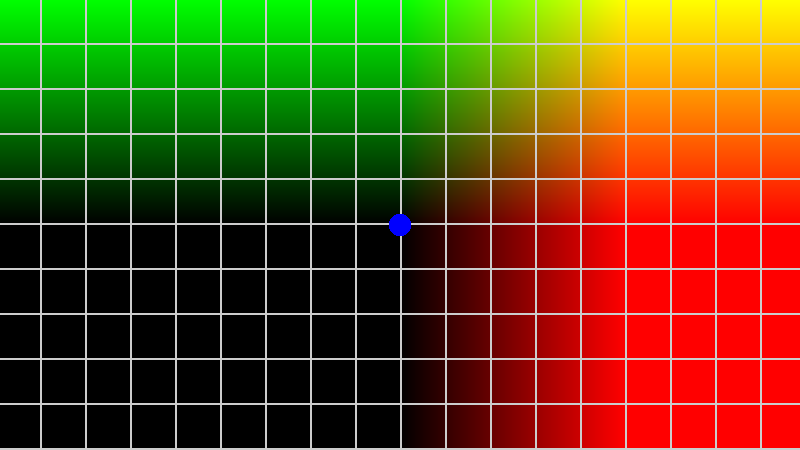
\includegraphics[width=\textwidth]{Plantilla-TFG-master/img/normY.png}
        \caption{Eje Y}
    \end{minipage}
    
    \medskip
    
    \begin{minipage}[b]{0.45\textwidth}
        \centering
        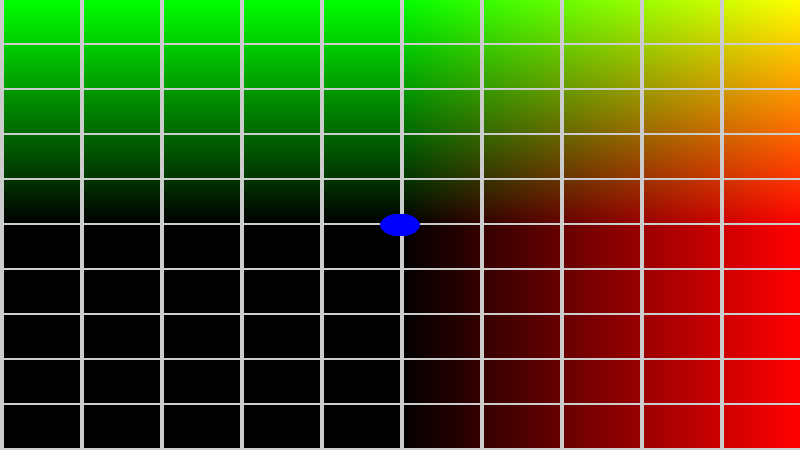
\includegraphics[width=\textwidth]{Plantilla-TFG-master/img/normXY.png}
        \caption{Ejes X e Y}
    \end{minipage}
    
    \caption{Normalización de coordenadas sobre distintos ejes}
    \label{fig:uv}
\end{figure}


\subsection{Generación de rayos primarios}
A partir de ahora, pensamos en nuestra escena no como en la que hemos definido el lienzo, sino aquella que queremos dibujar usando \textit{spheretracing} dada una función distancia con signo $\phi$. Esta escena estará definida en el espacio de coordenadas de mundo, el cual tiene un marco de referencia formado por tres vectores unitarios $B=\{e_x,e_y,e_z\}$ y un origen $o$, y colocaremos en ella los siguientes elementos (a partir de ahora supondremos que todas las tuplas de coordenadas son en coordenadas de mundo):
\begin{itemize}
    \item La \textbf{isosuperficie} $S_{\phi}$.
    \item \textbf{Plano de visión:} rejilla perpendicular al eje óptico de la cámara, donde cada uno de sus cuadrados corresponde a un píxel del lienzo.
    \item \textbf{Punto de la cámara $\boldsymbol{c_o}$:} punto del espacio desde donde se observa la escena.
    \item \textbf{Punto de atención o \textit{lookat point} $\boldsymbol{l}$:} hacia que punto del espacio debe mirar la cámara. En general tomaremos $l=o=(0,0,0)$.
\end{itemize}
La idea para conseguir representar la superficie consiste en trazar rayos a partir de $c_o$ hacia el centro de cada uno de los cuadrados del plano de visión, cada uno representando un píxel de la pantalla, de forma que si el rayo interseca con $S_\phi$ significa que ese píxel corresponde a un punto de la superficie, y será coloreado como tal.
\begin{figure}[h]
    \centering
    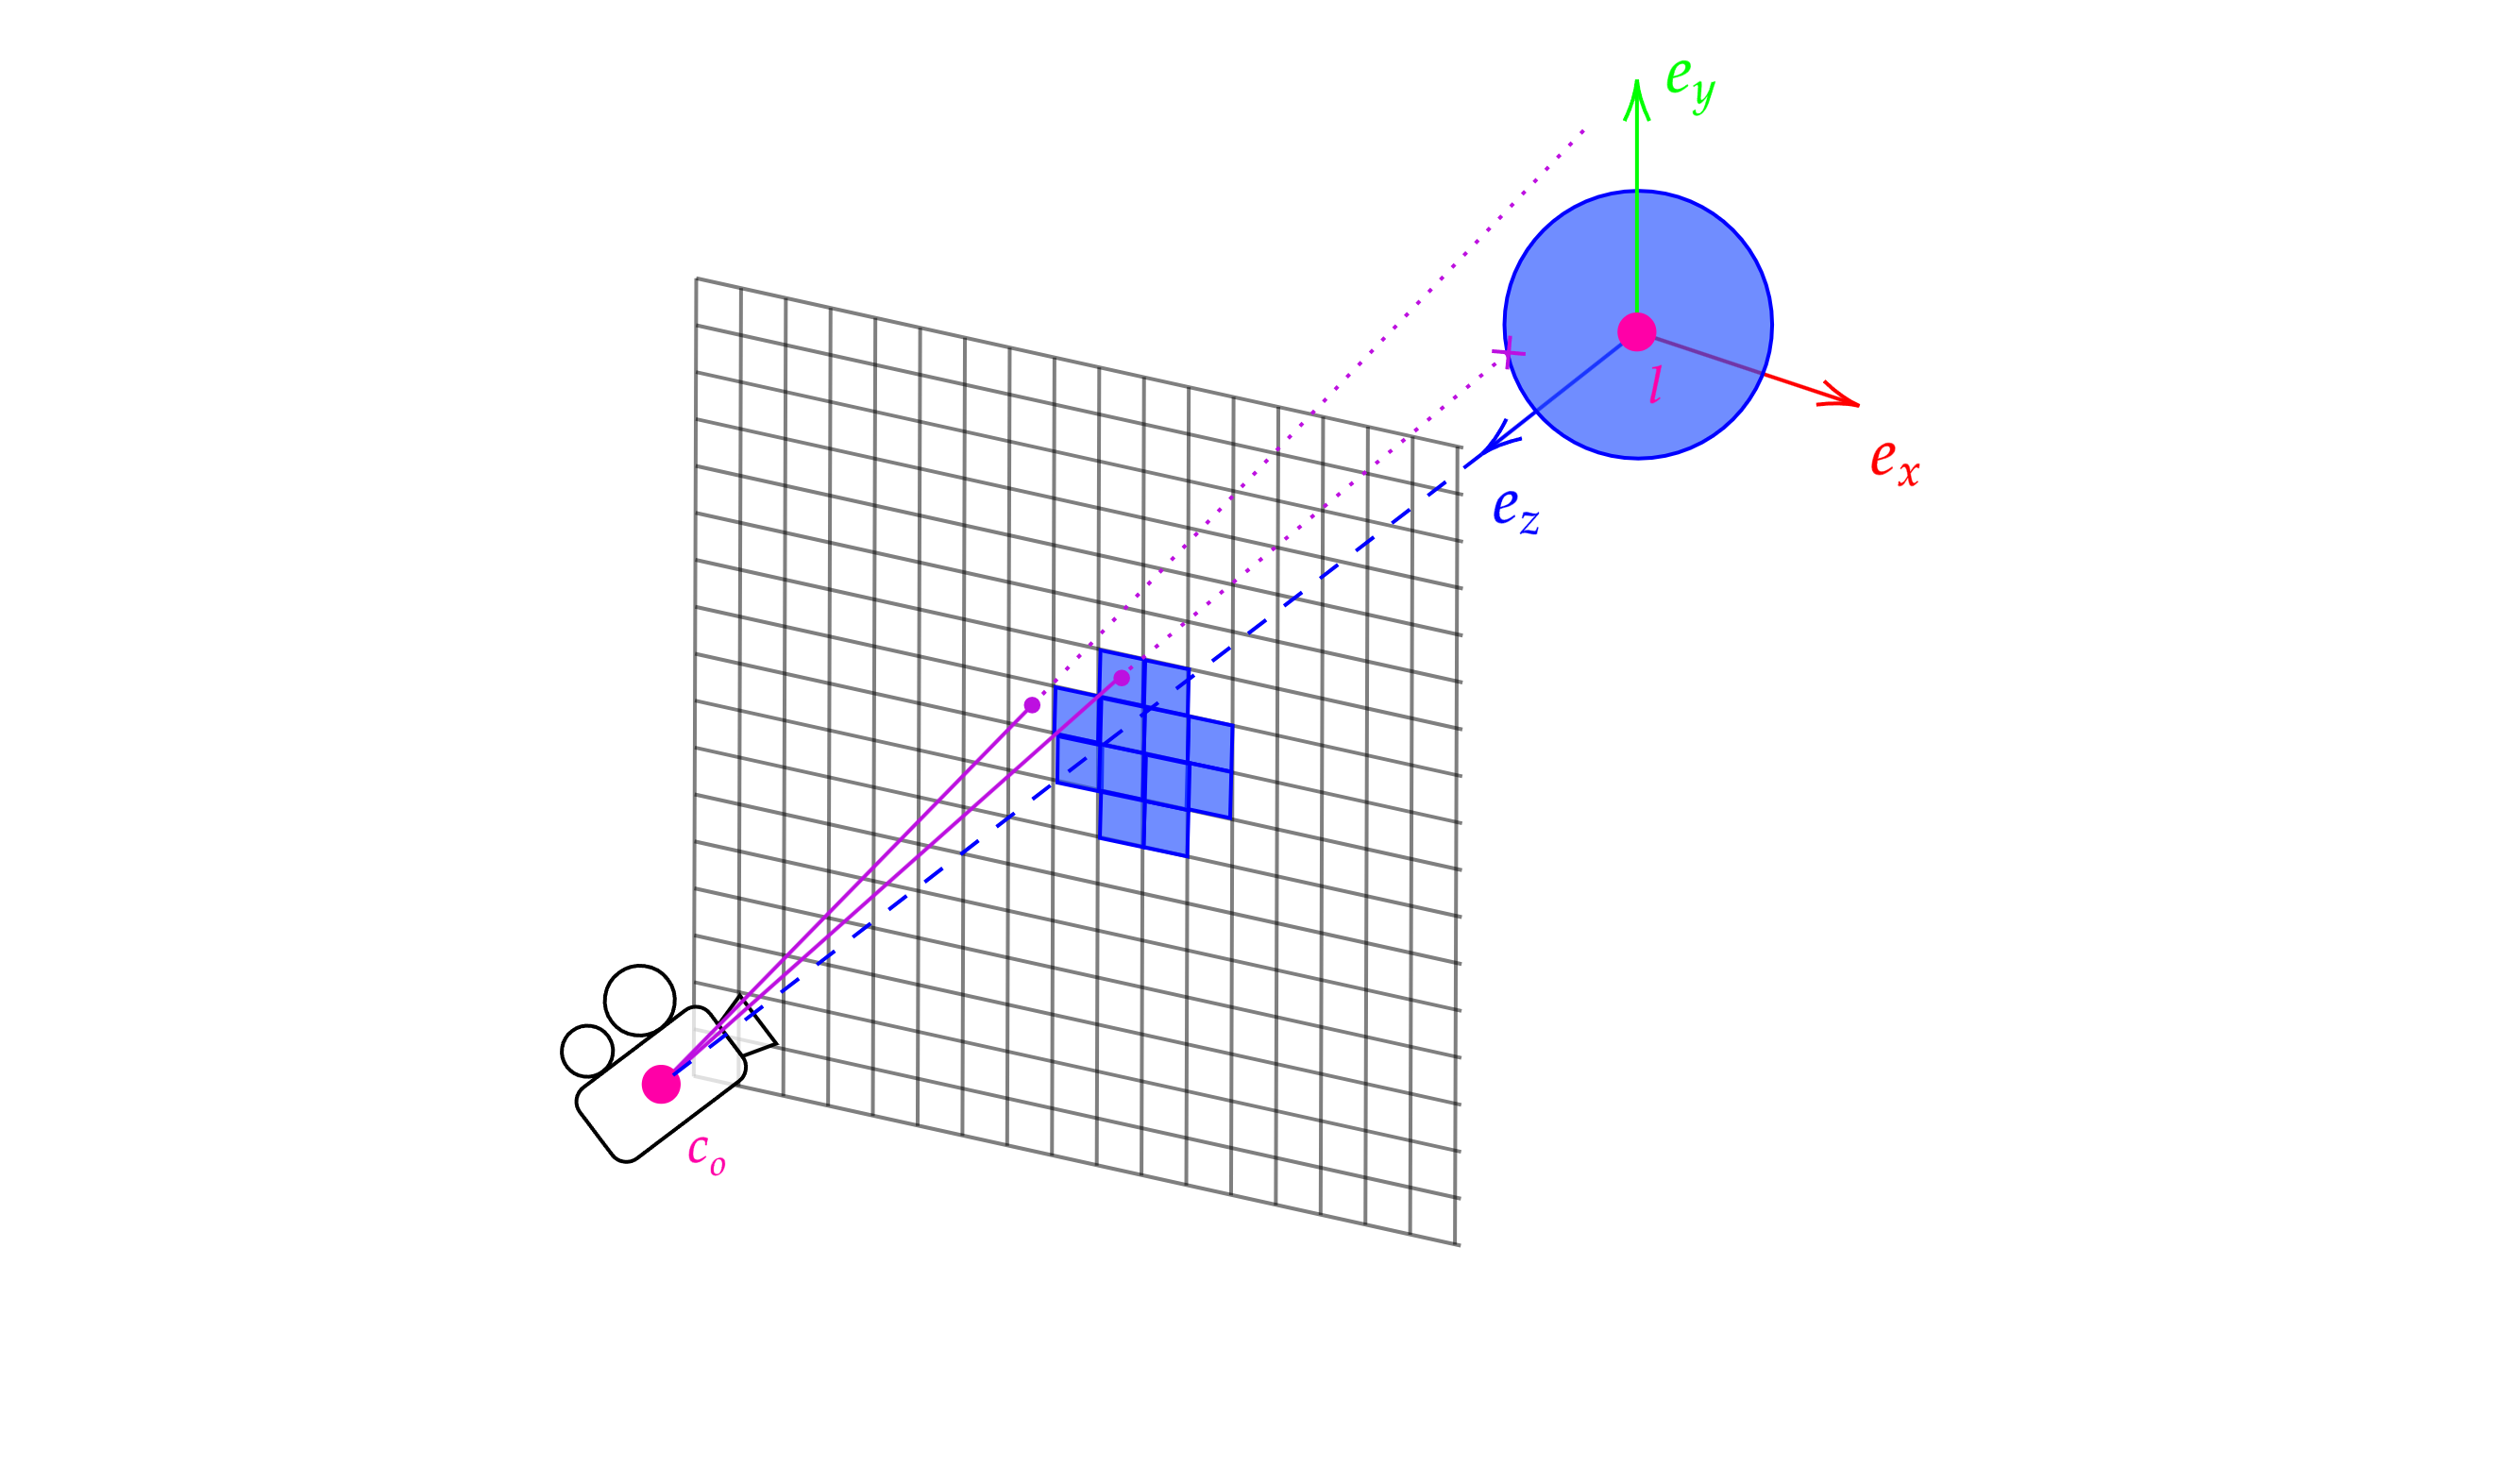
\includegraphics[width=\textwidth]{Plantilla-TFG-master/img/raymarch_fix.png}
    \caption{Trazado de rayos a través del plano de visión}
    \label{fig:raymarch1}
\end{figure}
\newline

Cada uno de estos rayos estará definido por un origen $r_o$ y una dirección $r_d$. El origen será siempre la posición de la cámara $c_o$, pero obtener la dirección requiere más trabajo. En el escenario descrito en la \autoref{fig:raymarch1}, donde $S_{\phi}$ es una esfera centrada en el origen y el observador se encuentra sobre el eje Z, dado que en todo momento conocemos las coordenadas de cada punto de la rejilla a través de $uv = (u,v)$, es claro que podemos tomar
$$r_d = (u,v,0) - c_0.$$ 
Una opción sería tomar $c_0 = (0,0,d)$, donde el valor $d$ es la distancia desde el punto del observador (foco de la proyección) al plano de visión. Modificar el valor de $d$ cambiaría los ángulos de apertura de visión horizontal y vertical, cambiando el tamaño aparente de los objetos proyectados. Es decir, $d$ actuaría como un control del campo de visión, de forma que cuanto mayor sea su valor mayores serán los ángulos de visión, y por tanto los objetos se verán más pequeños. Lo fijaremos a un valor de $1$. Sin embargo este escenario es el más sencillo posible, y si queremos poder mover la cámara manteniendo el punto de atención $l$ en el centro de la pantalla tendremos que poder trabajar con una orientación arbitraria suya. Para ello deberemos construir un marco de coordenadas de vista relativo a la cámara, que definiremos por una base ortonormal $\{f_1,f_2,f_3\}$ y el origen $c_0$.\newline

Para obtener el valor de los elementos de $f_1,f_2$ y $f_3$ empezamos obteniendo los siguientes vectores ortonormales.
\begin{itemize}
    \item \textbf{Vector director $\boldsymbol{c_d}$:} indica la dirección hacia la que mirará la cámara, que será paralela al eje $Z$ del marco de coordenadas de vista. Su valor vendrá dado por $c_d = l-c_o$.
    \item \textbf{\textit{Right vector} $\boldsymbol{c_r}$ }: paralelo al eje $X$ del marco de coordenadas de vista. Debe ser perpendicular tanto a $c_d$ como al vector \textit{view-up}. Este último, que denotaremos como $u$, es un vector libre que indica la dirección que el observador verá proyectada en vertical y apuntando hacia arriba en la imagen, y normalmente se toma el valor $u=(0,1,0)$ para que coincida con el eje $Y$. Al ser $c_r$ perpendicular al vector director y a \textit{view-up}, podemos obtenerlo como el producto vectorial de ambos: $c_r = u \times c_d$.
    \item \textbf{\textit{Up vector} $\boldsymbol{c_u}$}: paralelo al eje $Y$ del marco de coordenadas de vista. Como debe ser ortogonal a los otros dos, lo calculamos como $c_u = c_d\times c_r$.
\end{itemize}
A partir de estos vectores podemos obtener $\{f_1,f_2,f_3\}$ normalizándolos y teniendo en cuenta que el plano de visión y la cámara estarán orientados de forma opuesta:
\begin{equation*}
    f_1 = -\frac{c_r}{\Vert c_r\Vert} = -\frac{(0,1,0)\times c_d}{\Vert l-c_o\Vert},\quad 
    f_2 = \frac{c_u}{\Vert c_u\Vert } = f_3\times f_1, \quad
    f_3 = -\frac{c_d}{\Vert c_d\Vert} = -\frac{l-c_o}{\Vert l-c_o\Vert}. 
\end{equation*}
Ahora que tenemos el nuevo marco cartesiano, queda transformar el vector director original $r_d = (u,v,-1)$ a la base que acabamos de obtener. La matriz de cambio de base serán las coordenadas por columnas de $\{f_1,f_2,f_3\}$ escritas en función de $\{e_x,e_y,e_z\}$, que al ser la base del marco de coordenadas de mundo y al tratarse de una matriz de cambio de base entre dos marcos cartesianos, coincidirá con escribir por columnas $\{f_1,f_2,f_3\}$, de forma que
\begin{equation*}\label{eq:rayo}
    rayo = (u,v,-1)_{B}^t = \big(f_1\ \vert\  f_2\  \vert\  f_3\big) \cdot \begin{pmatrix}
        u\\
        v\\
        -1
    \end{pmatrix}.
\end{equation*}

\begin{figure}[ht!]
    \centering
    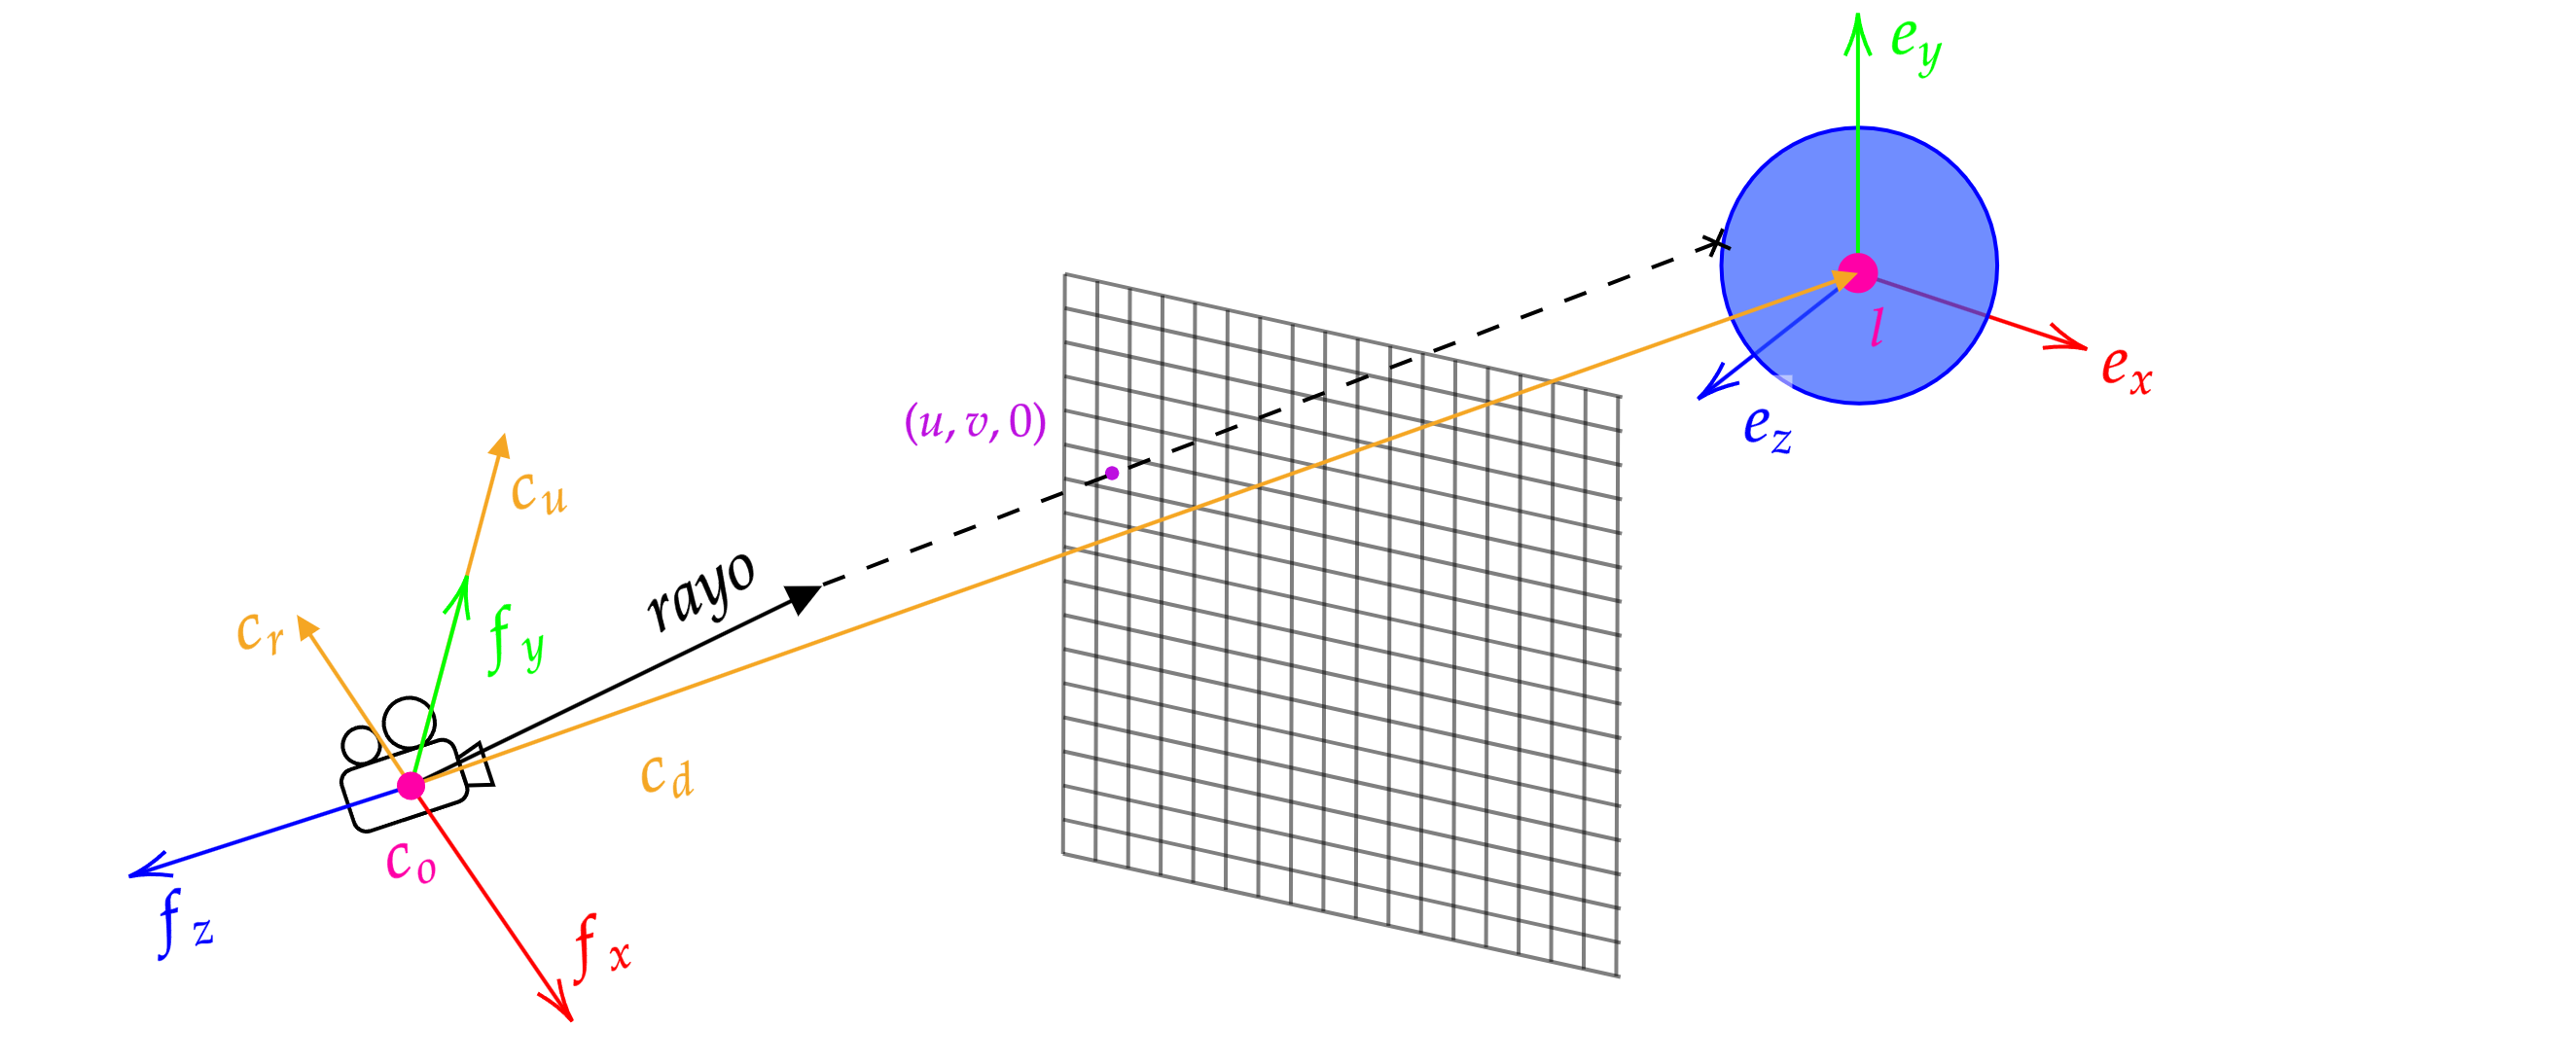
\includegraphics[width=\textwidth]{Plantilla-TFG-master/img/raydir_fix.png}
    \caption{Obtención de la dirección del rayo}
    \label{fig:raydir}
\end{figure}

\subsection{Algoritmos de intersección rayo-escena: \textit{raymarching} y \textit{spheretracing}}\label{sec:tracing}
Una vez que conocemos toda la información del rayo ya estamos en disposición de comprobar si este interseca con $S_{\phi}$. Para esto se pueden utilizar varios algoritmos, de entre los que estudiaremos el \textit{raymarching} y el \textit{spheretracing}. El método del \textit{spheretracing} es una variante del \textit{raymarching}, así que estudiaremos este primero.\newline

El \textbf{\textit{raymarching}} es un método iterativo: a partir de $c_o$, en cada iteración avanzamos en la dirección del rayo una distancia fija $\delta$. Evaluamos entonces nuestra SDF en la posición actual, de forma que si obtenemos un valor muy cercano a $0$ significará que hemos llegado a la isosuperficie. De lo contrario, repetimos el proceso hasta encontrar una intersección o superar un número máximo de iteraciones, en cuyo caso concluiremos que no hay intersección. La \autoref{a:raymarching} ilustra este procedimiento, donde \texttt{DibujarSuperficie()} y \texttt{DibujarFondo()} devuelven ternas RGBA que serán asignadas al píxel actual dependiendo de si hay intersección o no.\newline

\begin{figure}[ht!]
    \centering
    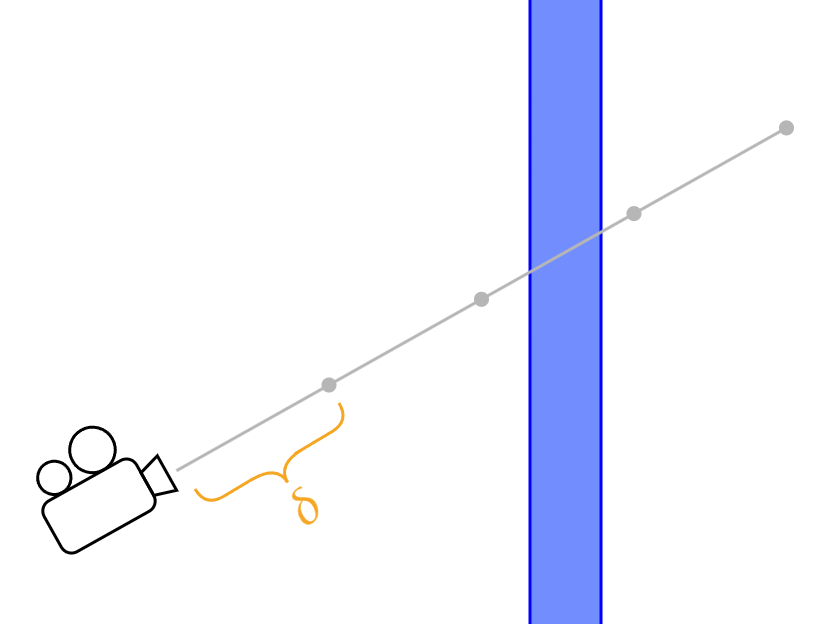
\includegraphics[width=0.4\textwidth]{Plantilla-TFG-master/img/miss.png}
    \caption{Pérdida de intersección en \textit{raymarching} para valores elevados de $\delta$}
    \label{fig:missInter}
\end{figure}

\SetKwComment{Comment}{// }{}
\begin{figure}[ht!]
    \centering
    \begin{minipage}{0.58\textwidth}
        \begin{algorithm}[H]
            \caption{Raymarching}
                \KwData{origen del rayo $c_o$, dirección del rayo $v$}
                \KwResult{terna RGB con el color del píxel actual}
                
                $d \gets 0$ \Comment{distancia total}
                
                \For{i $\in$ MAX\_ITERACIONES} {
                    $p \gets c_o +d\cdot v$
                    
                    sdf $\gets \phi(\text{p})$
                    
                    \If{sdf $< \varepsilon$}{
                       \Return{DibujarSuperficie($p,v,sdf$)}
                    }
            
                    $d\gets d + \delta$\;
            
                    \If{$d >$ MAX\_DISTANCIA}{
                        \Return{DibujarFondo()}
                    }
                }
        \end{algorithm}
    \end{minipage}%
    \hfill
    \begin{minipage}{0.4\textwidth}
        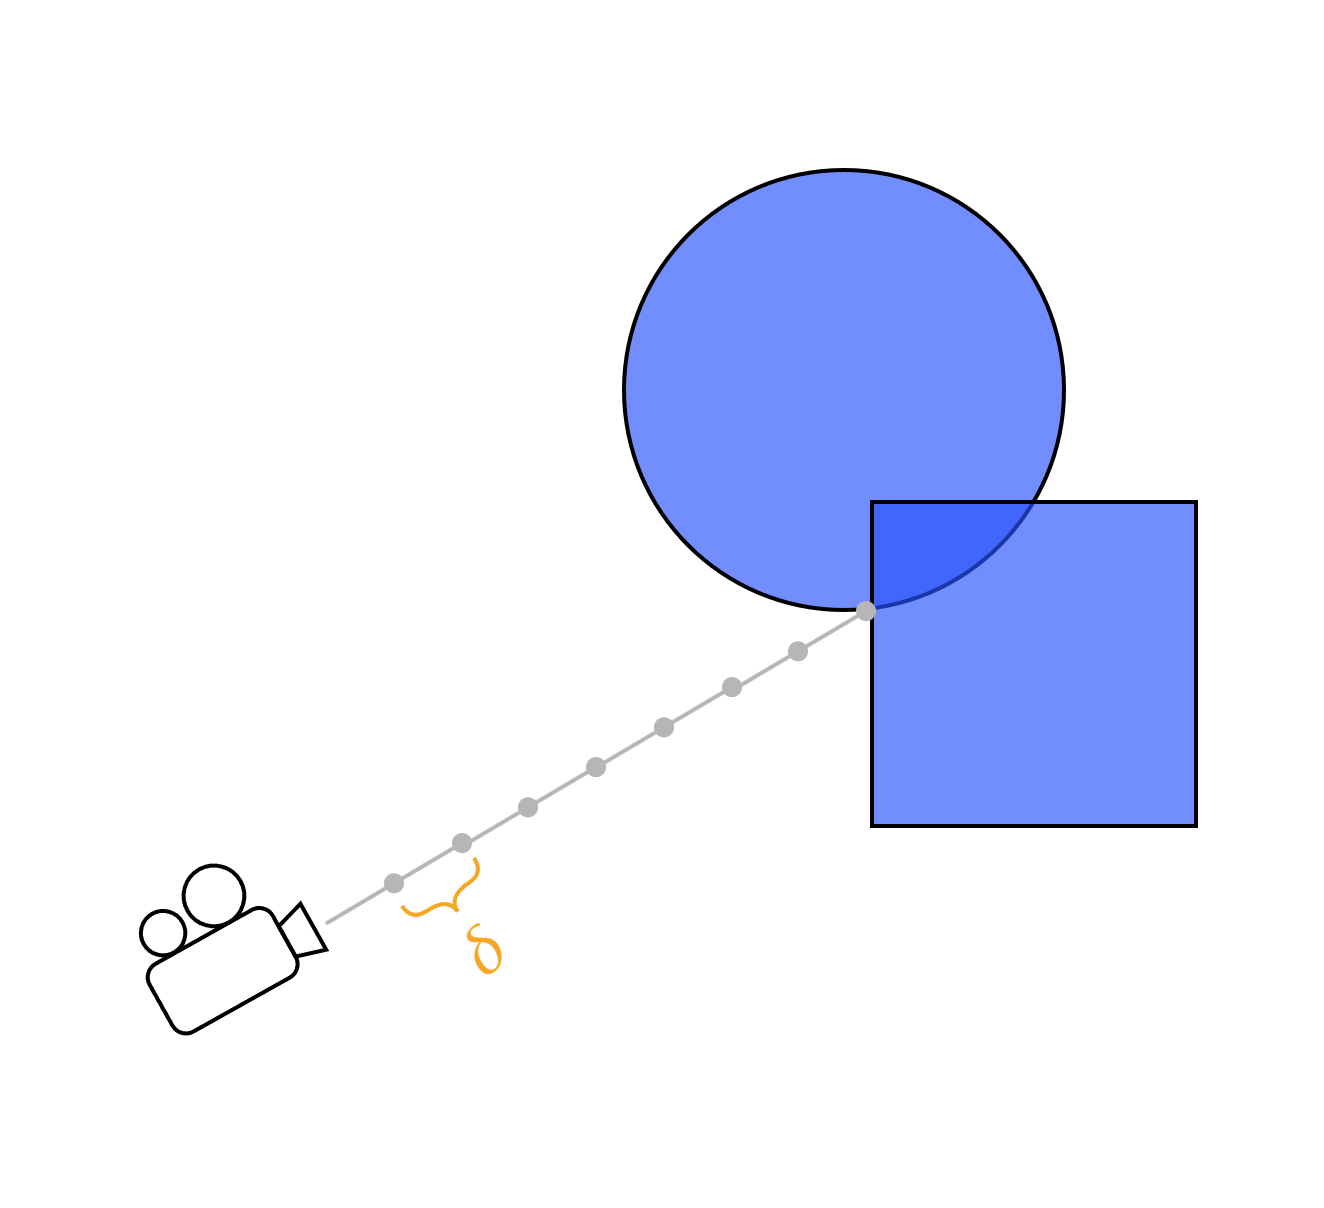
\includegraphics[width=\textwidth]{raymarching.png}
    \end{minipage}
    \caption{Algoritmo de \textit{raymarching}}
    \label{a:raymarching}
\end{figure}

Una desventaja de esta técnica es que puede ser bastante lenta, ya que cuanto más alejados estén los puntos de $S_\phi$ del observador, mayor es el número de iteraciones necesarias para encontrar la intersección en caso de que la haya. En el peor de los casos en el que tal intersección no exista, se habrá realizado el número máximo de iteraciones, que además será bastante alto debido a que el valor de incremento $\delta$ debe ser pequeño si no queremos perder ninguna intersección, como ocurre en la \autoref{fig:missInter}.\newline

Como solución a este problema aparece el \textit{spheretracing}, que reduce drásticamente el número de iteraciones, y por tanto de evaluaciones de $\phi$, necesarias para detectar la intersección. Su funcionamiento es similar al \textit{raymarching}, con la diferencia de que el incremento en la posición del rayo no es fija, sino que es la máxima que podemos tomar en cada momento asegurándonos de no perdernos una intersección. Esta distancia será la mínima del punto actual del rayo a $S_\phi$, que no es más que evaluar $\phi$ en dicho punto.\newline

Este será por tanto el algoritmo que utilizaremos para detectar qué pixels de la pantalla corresponden a la superficie $S_{\phi}$, y se encuentra descrito con detalle en la \autoref{a:spheretracing}. 
Con esto al fin podemos describir la forma que tendrá nuestro \textit{fragment shader} en la \autoref{fig:mainFS}. Claro está que esta versión todavía no es funcional, pues no sabemos qué forma tiene \texttt{DibujarSuperficie}, y como mucho podremos obtener una imagen que separe la isosuperficie del fondo usando colores planos como muestra la \autoref{fig:planos} para una esfera centrada en el origen. Veremos como mejorar esto en la próxima sección.

\begin{figure}[ht!]
    \centering
    \begin{minipage}{0.58\textwidth}
       \begin{algorithm}[H]
            \caption{Spheretracing}
                \KwData{origen del rayo $c_o$, dirección del rayo $v$}
                \KwResult{terna RGB con el color del píxel actual}
                $d \gets 0$ \Comment{distancia actual}
                
                \For{i $\in$ MAX\_ITERACIONES} {
                    $p \gets c_o + d \cdot v$
                    
                    $sdf \gets \phi(p)$
                    
                    \If{sdf $< \varepsilon$}{
                       \Return{$DibujarSuperficie(p,v,sdf)$}
                    }
            
                    $d \gets$ d + sdf
            
                    \If{$d >$ MAX\_DISTANCIA}{
                        \Return{$DibujarFondo()$}
                    }
                }
        \end{algorithm}
    \end{minipage}%
    \hfill
    \begin{minipage}{0.4\textwidth}
        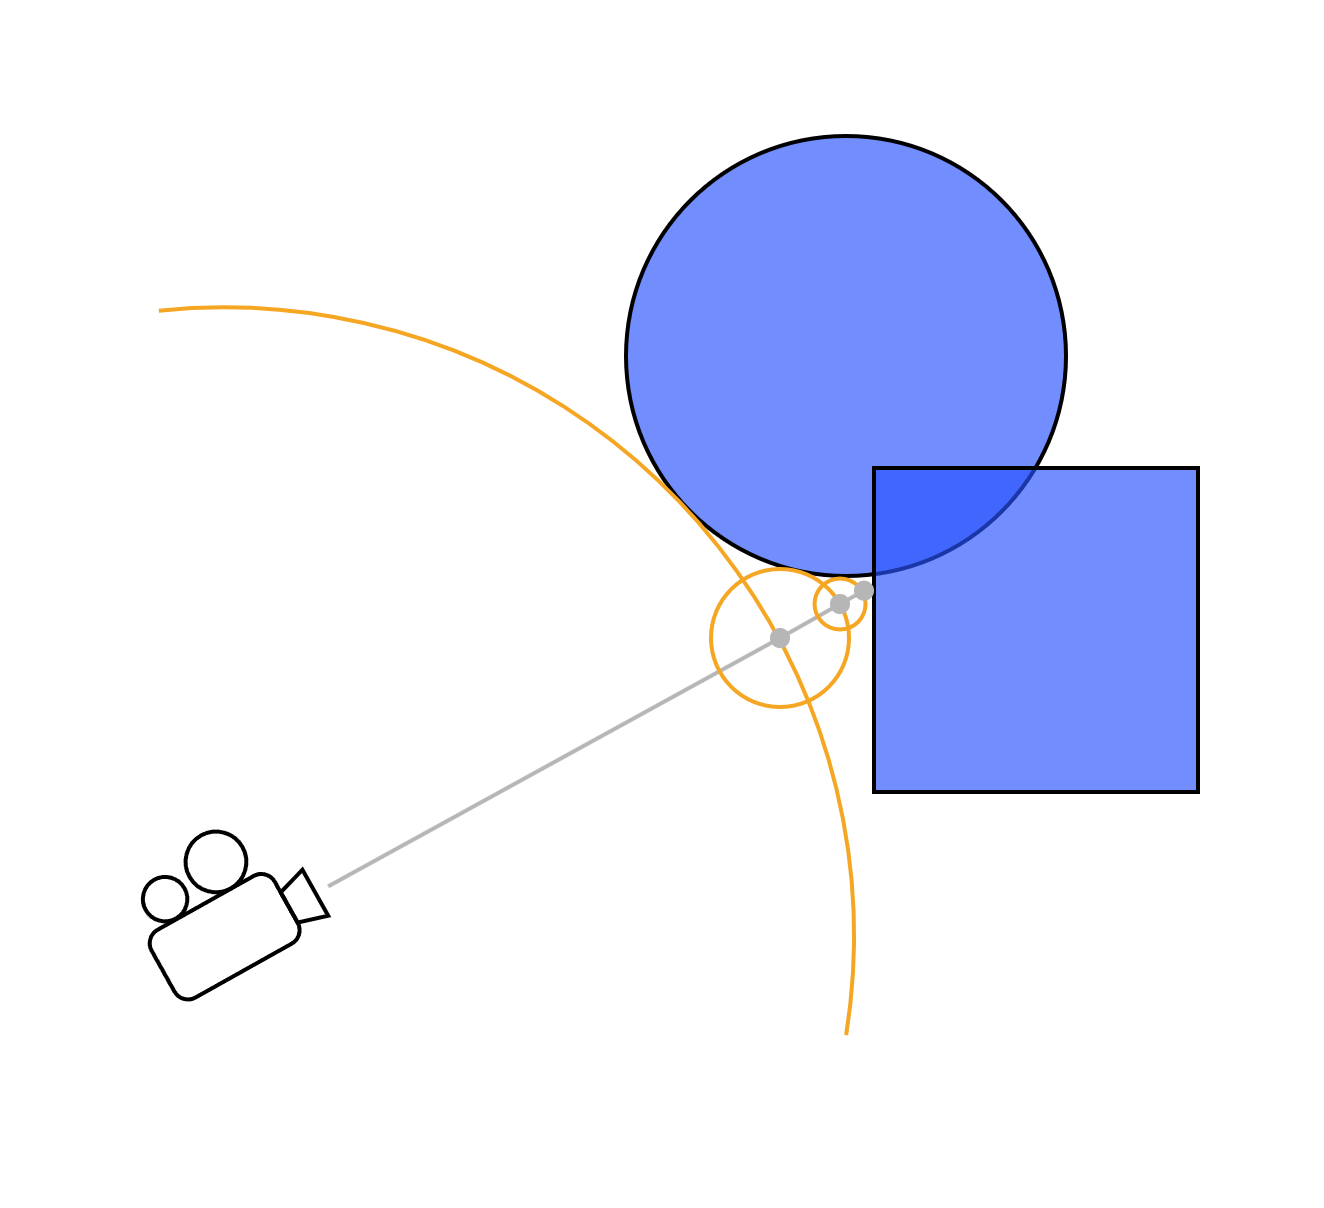
\includegraphics[width=\textwidth]{spheremarching.png}
    \end{minipage}
    \caption{Algoritmo de \textit{spheretracing}}
    \label{a:spheretracing}
\end{figure}

\begin{figure}[ht!]
    \centering
    
       \begin{algorithm}[H]
            \caption{Fragment Shader}
            \KwData{coordenadas de dispositivo $v_{frag}$ del píxel actual}
            \KwResult{color del píxel actual como terna RGBA $v_{col}$}

                $c_0 \gets $ posición de cámara en función de la entrada del ratón

                $l\gets $ punto de atención elegido por el usuario
                
                $uv \gets 2\cdot \frac{v_{frag} - 0.5\cdot u\_resolution}{u\_resolution_y}$\\[5pt]

                $f_1,\ f_2,\ f_3 \gets CalcularMarcoCartesiano(c_0, l)$
                
                $r_d \gets (f_1\ \vert \ f_2\ \vert \ f_3)\cdot normalizar ((uv_x, uv_y,-1))$\\[5pt]

                $color \gets$ spheretracing$(c_0, r_d)$\\[5pt]

                $v_{col} \gets (color_x, color_y, color_z, 1)$
        \end{algorithm}
    \caption{Cuerpo del método \texttt{main} del \textit{fragment shader}}
    \label{fig:mainFS}
\end{figure}


\begin{figure}[ht!]
    \centering
    
\includegraphics[width=0.8\textwidth]{Plantilla-TFG-master/img/escenaPlana.png}
    \caption{Resultado de \textit{spheretracing} asignando colores planos}
    \label{fig:planos}
\end{figure}
